\section{Atividade 10}

\subsection{Identificação de Sistemas}

Nesta atividade, abordamos a identificação do sistema representado pela função de transferência especificada na Atividade 3. Utilizando a resposta ao degrau unitário, aplicamos os métodos de Harriot e Smith para identificar os parâmetros de um sistema de segunda ordem. Os resultados obtidos por cada método serão comparados para determinar qual fornece uma identificação mais precisa das características do sistema.

Para otimizar a análise e assegurar que os resultados sejam imediatamente interpretáveis, adotamos um degrau de entrada com amplitude 5. Este ajuste estratégico evita a complexidade associada à normalização posterior dos dados, garantindo que a amplitude da resposta permaneça normalizada em 1 ao longo do tempo.

A Figura \ref{fig:diagrama-sistema} ilustra a resposta ao degrau unitário do sistema massa-mola-amortecedor, especificado pelos parâmetros \(M = 10\), \(C = 7\), e \(K = 5\). Essa resposta é crucial para a identificação dos parâmetros do sistema utilizando os métodos de Harriot e Smith, permitindo uma análise detalhada da dinâmica do sistema em resposta a perturbações externas.

\begin{figure}[h]
    \centering
    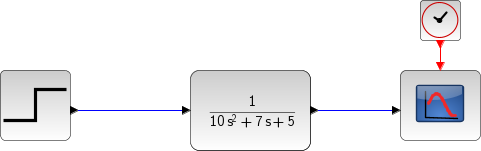
\includegraphics[width=0.8\textwidth]{atividades/10-atividade/assets/diagrama-sistema.png}
    \caption{Resposta ao degrau unitário do sistema massa-mola-amortecedor.}
    \label{fig:diagrama-sistema}
\end{figure}

Utilizando a ferramenta DataTip, marcamos pontos significativos na curva de resposta correspondentes a 20\%, 60\%, 73\% e 100\% do valor final. Estes pontos são essenciais para a aplicação dos métodos de identificação, pois fornecem dados precisos sobre a resposta do sistema em diferentes fases do seu comportamento transitório.

A Figura \ref{fig:sistema-identificado-forcado-normalizado} apresenta a resposta ao degrau unitário com os parâmetros identificados segundo os métodos de Harriot e Smith, destacando a utilidade dessas metodologias na análise de sistemas dinâmicos.

\begin{figure}[h]
    \centering
    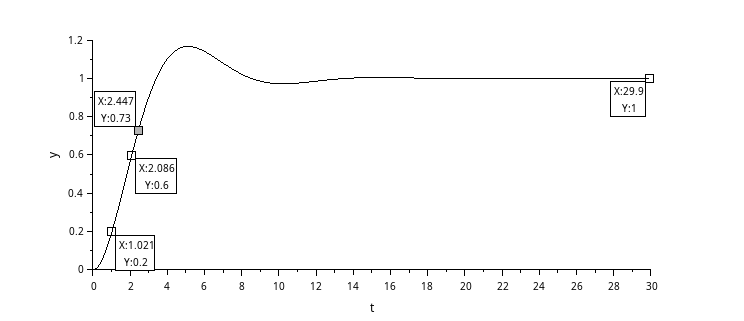
\includegraphics[width=0.8\textwidth]{atividades/10-atividade/assets/sistema-identificado-forcado-normalizado.png}
    \caption{Identificação dos parâmetros do sistema com a resposta ao degrau unitário, ilustrando a eficácia dos métodos de Harriot e Smith.}
    \label{fig:sistema-identificado-forcado-normalizado}
\end{figure}

\subsection{Aplicação do Método de Harriot}

O Método de Harriot é tradicionalmente empregado para identificar os parâmetros de sistemas de primeira ordem, focando na constante de tempo (\(\tau\)) e no ganho do sistema (\(K\)). Este método analisa como o sistema responde a um degrau unitário para extrair esses parâmetros. Para esta análise específica, optou-se por aplicar um degrau de amplitude 5, facilitando a interpretação dos resultados ao evitar a normalização posterior. Duas abordagens principais foram consideradas:

\begin{enumerate}
    \item \textbf{Utilização direta do degrau de amplitude 5:} Esta abordagem aproveita a amplitude do degrau para manter os dados experimentais alinhados com o sistema real, sem a necessidade de ajustes adicionais para a normalização.
    \item \textbf{Normalização para um degrau unitário:} Caso um degrau unitário tivesse sido aplicado, seria necessário normalizar os valores de resposta dividindo-os pelo valor final esperado (\(5K\)), adaptando a análise às fórmulas padrão do Método de Harriot.
\end{enumerate}

\subsubsection{Cálculo da Constante de Tempo}

A constante de tempo crítica para a aplicação do Método de Harriot foi determinada como segue:
\[
    \tau = 0.5 \cdot \frac{t_{73}}{1.3} = 0.5 \cdot \frac{2.449}{1.3} \approx 0.9419 \text{ segundos}
\]

Os pontos de resposta ao degrau usados para esta análise incluem:
\begin{itemize}
    \item \(X = 1.022\), \(Y = 0.2\) (20\% do valor final).
    \item \(X = 2.094\), \(Y = 0.6\) (60\% do valor final).
    \item \(X = 2.449\), \(Y = 0.73\) (73\% do valor final).
    \item \(X = 29.9\), \(Y = 1\) (100\% do valor final).
\end{itemize}

\subsubsection{Limitação do Método de Harriot}

Uma limitação significativa do Método de Harriot é sua aplicabilidade principalmente a sistemas sobreamortecidos. No entanto, o sistema em análise é subamortecido. Além disso, para uma eficaz aplicação do método, a razão \(Y/KM\) deve ser maior que 0.26 após a normalização para uma resposta ao degrau unitário. No presente caso, o valor de \(Y/KM\) calculado foi 0.175, indicando que o Método de Harriot não é adequado para esta configuração específica. Portanto, são recomendadas abordagens alternativas de identificação ou ajustes na configuração experimental.

\begin{figure}[h]
    \centering
    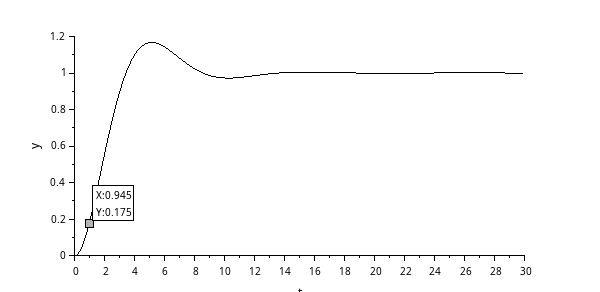
\includegraphics[width=0.8\textwidth]{atividades/10-atividade/assets/sistema-t73-identificado-nromalizacao-forcada.png}
    \caption{Identificação do sistema massa-mola-amortecedor utilizando o Método de Harriot.}
    \label{fig:sistema-t73-identificado-nromalizacao-forcada}
\end{figure}

A Figura \ref{fig:sistema-t73-identificado-nromalizacao-forcada} ilustra a tentativa de aplicação do Método de Harriot, destacando que a inadequação dos parâmetros extraídos confirma as limitações do método para este caso específico. Esta análise sugere a necessidade de explorar métodos alternativos que sejam mais compatíveis com as características dinâmicas do sistema subamortecido em estudo.

\subsection{Aplicação do Método de Smith}

O Método de Smith é uma técnica avançada que utiliza a resposta ao degrau unitário para estimar a frequência natural (\(\omega_n\)) e o fator de amortecimento (\(\zeta\)) de um sistema. Este método é particularmente útil para a análise de sistemas de segunda ordem, proporcionando uma visão clara das características dinâmicas do sistema a partir de sua resposta temporal.

\subsubsection{Análise de Razão Temporal}

Inicialmente, calculamos a razão entre os tempos que correspondem a 20\% e 60\% da resposta final do degrau. A razão é calculada usando a fórmula:
\[
    \frac{t_{20}}{t_{60}} = \frac{1.022}{2.086} \approx 0.461706
\]
Esta métrica é crucial porque define a trajetória no gráfico de Smith para deduzir os valores de \(\zeta\) e \(\tau\).

\subsubsection{Interpretação Gráfica}

Utilizando a razão calculada, consultamos o gráfico do Método de Smith, conforme ilustrado na Figura \ref{fig:analise-smith}. Este gráfico correlaciona \(\frac{t_{20}}{\tau}\) e \(\frac{t_{60}}{\tau}\) com os valores de \(\zeta\) e \(\tau\), facilitando a interpretação direta das características do amortecimento e da constante de tempo do sistema. É importante notar que o gráfico apresenta dois eixos Y: o da esquerda mostra \(\frac{t_{60}}{\tau}\) enquanto o da direita exibe valores para \(\zeta\).

\begin{figure}[h]
    \centering
    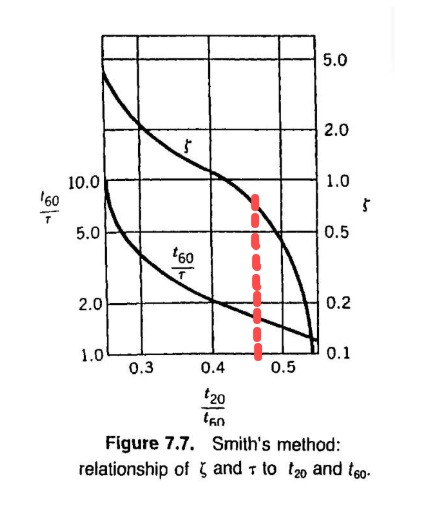
\includegraphics[width=0.8\textwidth]{atividades/10-atividade/assets/analise-smith.png}
    \caption{Gráfico utilizado no Método de Smith: relação entre \(\zeta\) e \(\tau\) com \(\frac{t_{20}}{\tau}\) e \(\frac{t_{60}}{\tau}\).}
    \label{fig:analise-smith}
\end{figure}

Através deste gráfico, identificamos que a razão \(\frac{t_{60}}{\tau}\) para nossa razão específica \(\frac{t_{20}}{t_{60}}\) é aproximadamente 1.8. Com esta informação, podemos calcular \(\tau\) usando o tempo conhecido \(t_{60}\):
\[
    \tau = \frac{t_{60}}{1.8} = \frac{2.086}{1.8} \approx 1.159 \text{ segundos}
\]

\subsubsection{Cálculo de Parâmetros do Sistema}

Com o \(\tau\) calculado, podemos inferir \(\zeta\) diretamente do gráfico e aplicar esses valores na função de transferência do sistema:
\[
    G(s) = \frac{Kp}{\tau^2 s^2 + 2 \zeta \tau s + 1} = \frac{Kp}{(1.159)^2 s^2 + 2 \zeta (1.159) s + 1}
\]

\subsubsection{Limitações e Recomendações}

A análise conduzida através do Método de Smith, apesar de instrutiva, enfrenta limitações significativas devido ao uso de uma representação gráfica baseada em imagem. A precisão dos valores obtidos pode ser comprometida por ruídos visuais e erros de interpretação. Para resultados mais confiáveis, é recomendável o uso de gráficos dinâmicos gerados diretamente de dados experimentais, minimizando a interpretação visual e os erros associados.


\subsection{Comparação dos Métodos e Conclusão}

A avaliação dos métodos de Harriot e Smith revelou nuances importantes no processo de identificação de sistemas. Cada método demonstra forças e limitações que são cruciais ao considerar a adequação ao tipo específico de sistema analisado.

\subsubsection{Método de Harriot}
O Método de Harriot, tradicionalmente adequado para sistemas sobreamortecidos, encontrou dificuldades significativas de aplicação ao sistema subamortecido em estudo. Além disso, o indicador chave para a aplicação do método, a razão \(Y/KM\), mostrou-se insuficiente (\(0.175\)), ficando bem abaixo do limite necessário (\(0.26\)) para uma identificação eficaz. Isso sugere que o Método de Harriot pode não ser a escolha ideal para sistemas que não se enquadram claramente em configurações sobreamortecidas, ou quando a resposta ao degrau não alcança um platô claro e definido.

\subsubsection{Método de Smith}
O Método de Smith, por outro lado, é mais flexível para sistemas subamortecidos, oferecendo insights sobre a frequência natural e o fator de amortecimento. No entanto, a análise dependente de uma representação gráfica visual introduz um nível de incerteza, especialmente quando os dados são interpretados a partir de uma imagem estática, que pode incorporar ruídos e distorções visuais. Tais fatores podem afetar a precisão dos parâmetros inferidos, limitando a confiabilidade das conclusões.

\subsubsection{Considerações Finais e Recomendações}
Em face das análises realizadas e das limitações observadas em ambos os métodos, conclui-se que a identificação dos parâmetros do sistema não foi alcançada de maneira confiável e satisfatória. As incertezas e as inadequações metodológicas levam à recomendação de que outras abordagens sejam consideradas para uma identificação mais precisa. Métodos alternativos, possivelmente combinando aspectos quantitativos e qualitativos, ou mesmo ajustes na configuração experimental, podem ser necessários para garantir resultados mais robustos e verificáveis.

Concluímos que, diante das circunstâncias e resultados, é mais prudente não afirmar com certeza a identificação dos parâmetros do sistema. Em vez disso, recomenda-se explorar outras técnicas e metodologias, talvez integrando dados adicionais ou utilizando software de simulação avançada, para obter uma compreensão mais profunda e precisa das dinâmicas do sistema.

Este caso destaca a importância de escolher o método apropriado para o tipo de sistema e resposta observada e sugere que a cautela seja um componente crucial ao interpretar e aplicar técnicas de identificação em engenharia de controle.
